\documentclass[11pt,a4paper]{report}
\usepackage[textwidth=37em,vmargin=30mm]{geometry}
\usepackage{calc,xunicode,amsmath,amssymb,paralist,enumitem,tabu,booktabs,datetime2,xeCJK,xeCJKfntef,listings}
\usepackage{tocloft,fancyhdr,tcolorbox,xcolor,graphicx,eso-pic,xltxtra,xelatexemoji}

\newcommand{\envyear}[0]{2025}
\newcommand{\envdatestr}[0]{2025-09-22}
\newcommand{\envfinaldir}[0]{webdb/2025/20250922/final}

\usepackage[hidelinks]{hyperref}
\hypersetup{
    colorlinks=false,
    pdfpagemode=FullScreen,
    pdftitle={Web Digest - \envdatestr}
}

\setlength{\cftbeforechapskip}{10pt}
\renewcommand{\cftchapfont}{\rmfamily\bfseries\large\raggedright}
\setlength{\cftbeforesecskip}{2pt}
\renewcommand{\cftsecfont}{\sffamily\small\raggedright}

\setdefaultleftmargin{2em}{2em}{1em}{1em}{1em}{1em}

\usepackage{xeCJK,xeCJKfntef}
\xeCJKsetup{PunctStyle=plain,RubberPunctSkip=false,CJKglue=\strut\hskip 0pt plus 0.1em minus 0.05em,CJKecglue=\strut\hskip 0.22em plus 0.2em}
\XeTeXlinebreaklocale "zh"
\XeTeXlinebreakskip = 0pt


\setmainfont{Brygada 1918}
\setromanfont{Brygada 1918}
\setsansfont{IBM Plex Sans}
\setmonofont{JetBrains Mono NL}
\setCJKmainfont{Noto Serif CJK SC}
\setCJKromanfont{Noto Serif CJK SC}
\setCJKsansfont{Noto Sans CJK SC}
\setCJKmonofont{Noto Sans CJK SC}

\setlength{\parindent}{0pt}
\setlength{\parskip}{8pt}
\linespread{1.15}

\lstset{
	basicstyle=\ttfamily\footnotesize,
	numbersep=5pt,
	backgroundcolor=\color{black!5},
	showspaces=false,
	showstringspaces=false,
	showtabs=false,
	tabsize=2,
	captionpos=b,
	breaklines=true,
	breakatwhitespace=true,
	breakautoindent=true,
	linewidth=\textwidth
}






\newcommand{\coverpic}[2]{
    % argv: itemurl, authorname
    Cover photo by #2~~(\href{#1}{#1})
}
\newcommand{\makeheader}[0]{
    \begin{titlepage}
        % \newgeometry{hmargin=15mm,tmargin=21mm,bmargin=12mm}
        \begin{center}
            
            \rmfamily\scshape
            \fontspec{BaskervilleF}
            \fontspec{Old Standard}
            \fontsize{59pt}{70pt}\selectfont
            WEB\hfill DIGEST
            
            \vfill
            % \vskip 30pt
            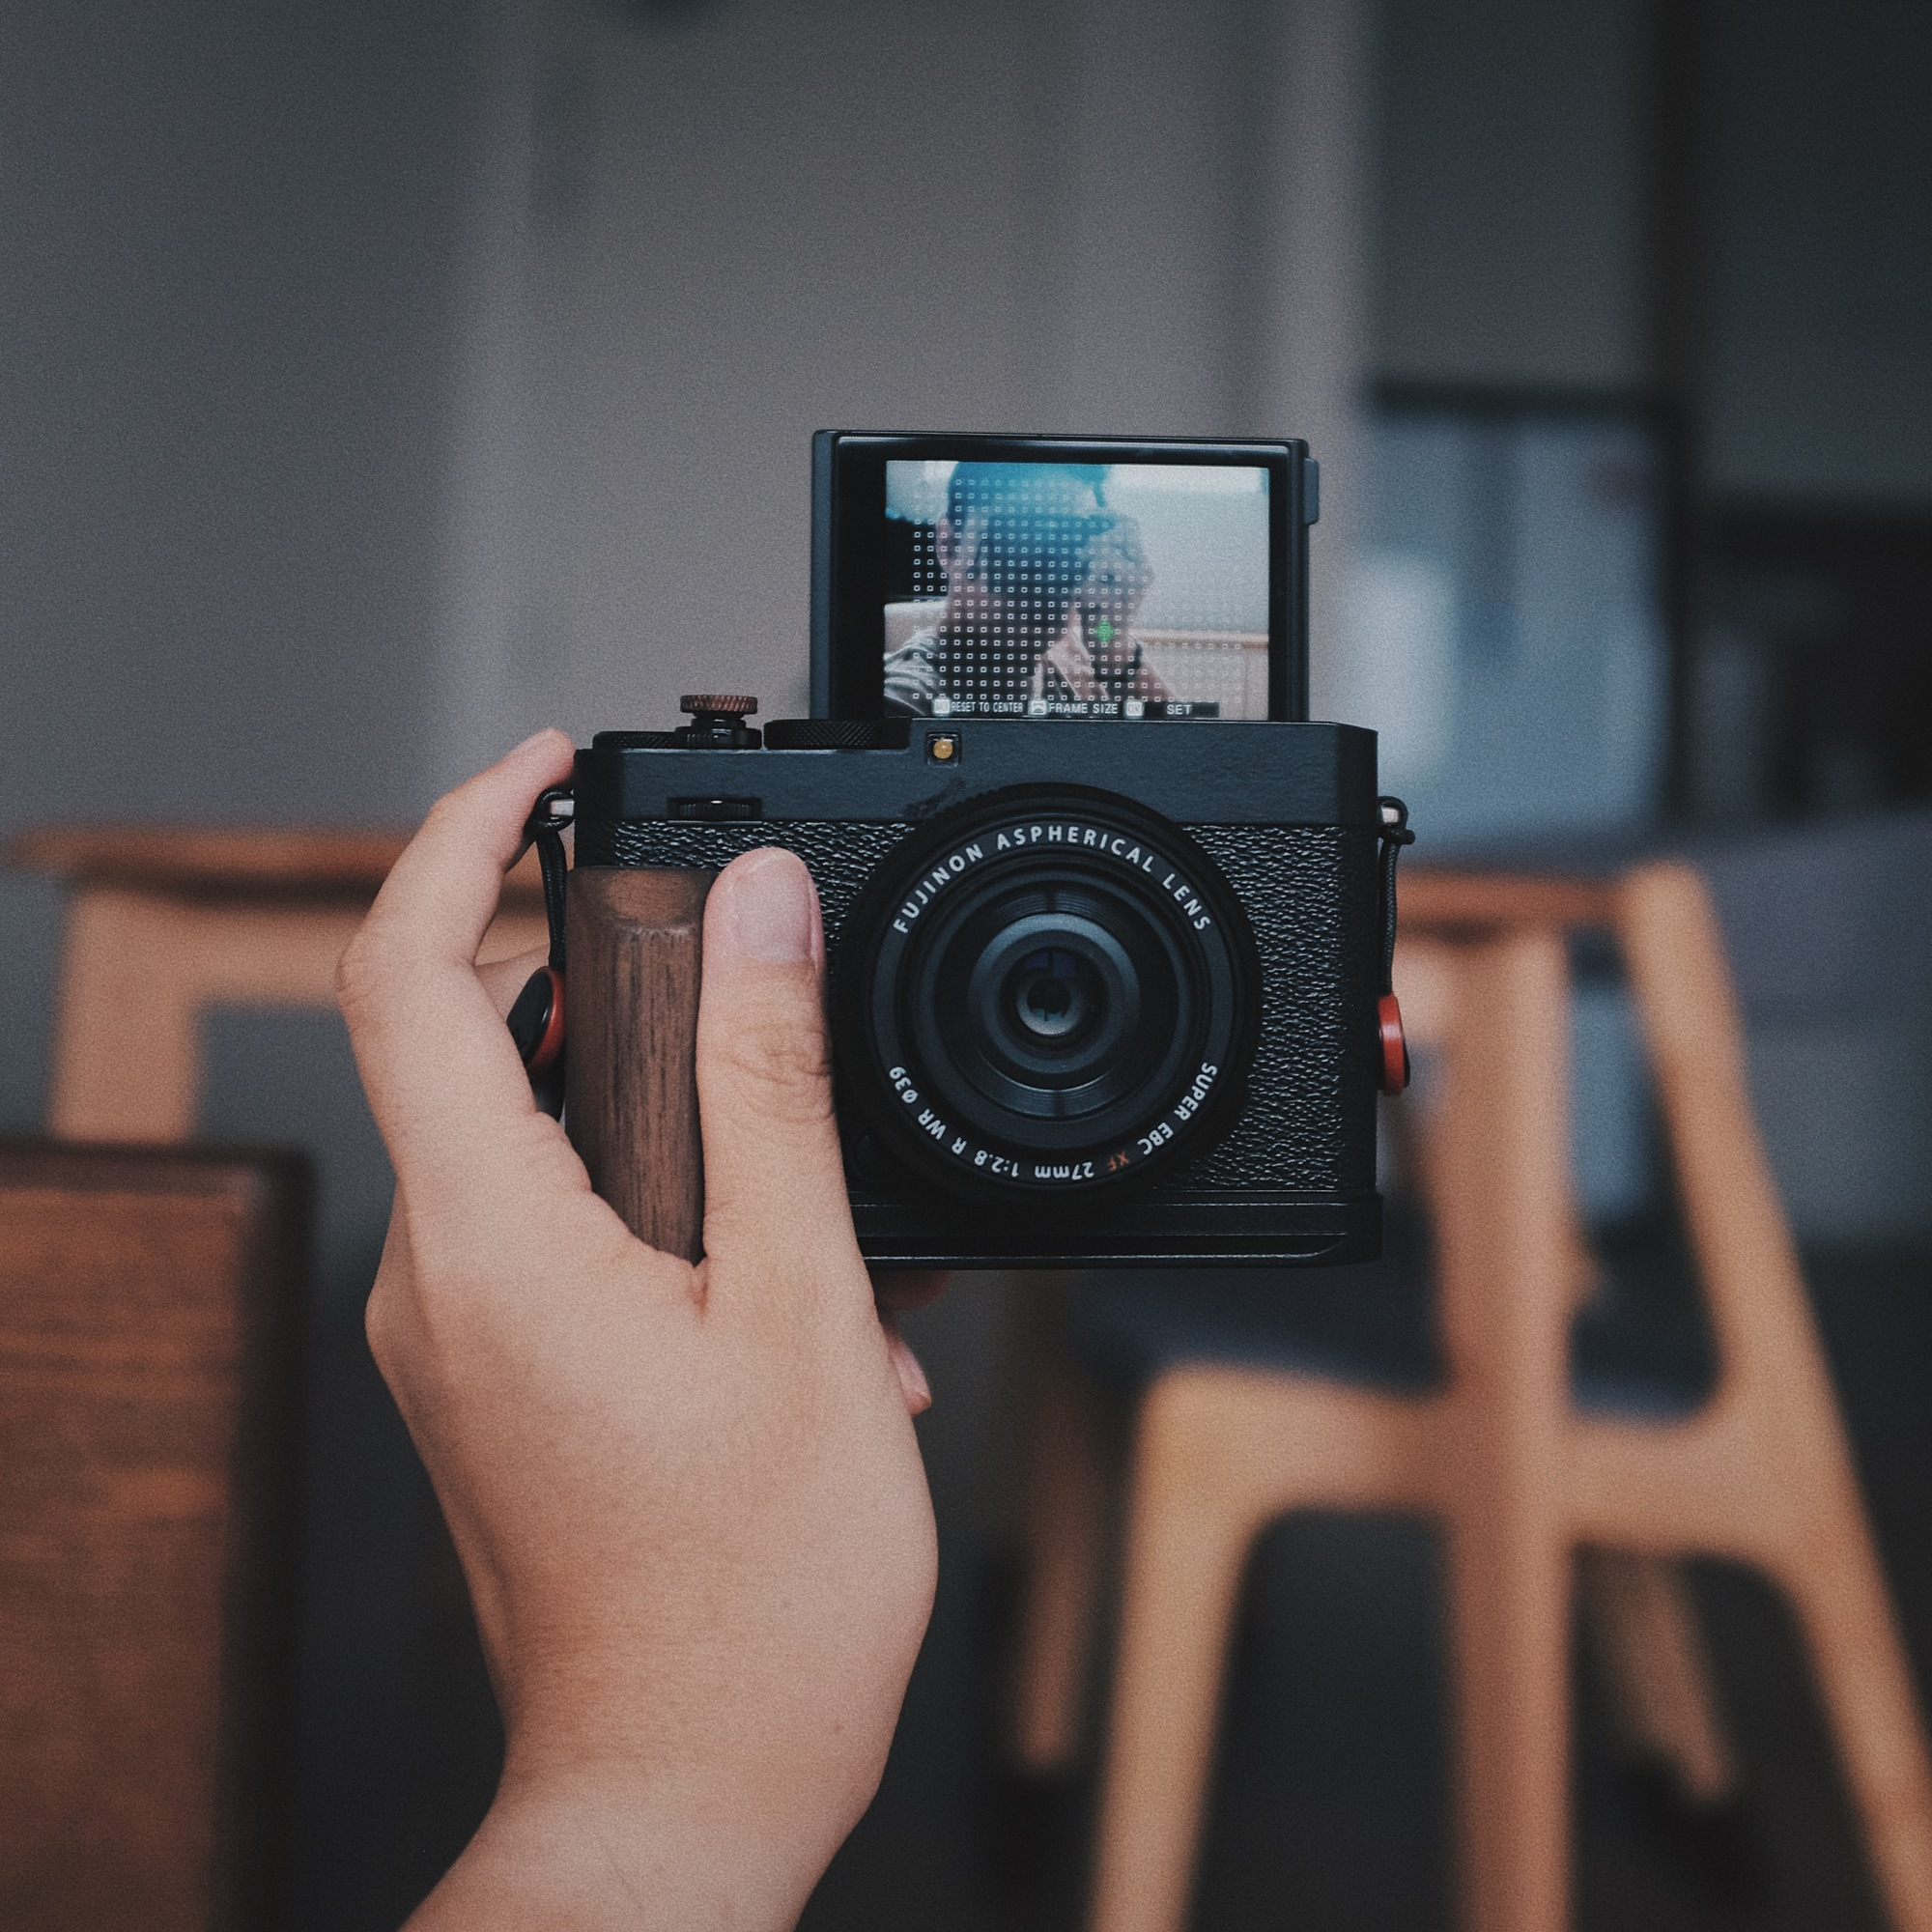
\includegraphics[width=\linewidth]{\envfinaldir/coverpic-prod.jpg}\par
            % \vskip 30pt
            \vfill

            \normalsize\rmfamily\scshape
            \copyright{} The Web Digest Project \hfill\large \envdatestr
        \end{center}
    \end{titlepage}
    % \restoregeometry
}
\newcommand{\simplehref}[1]{%
    \textcolor{blue!80!green}{\href{#1}{#1}}%
}
\renewcommand{\contentsname}{\center\Huge\sffamily\bfseries Contents\par\vskip 20pt}
\newcounter{ipartcounter}
\setcounter{ipartcounter}{0}
\newcommand{\ipart}[1]{
    % \vskip 20pt
    \clearpage
    \stepcounter{ipartcounter}
    \phantomsection
    \addcontentsline{toc}{chapter}{#1}
    % \begin{center}
    %     \Huge
    %     \sffamily\bfseries
    %     #1
    % \end{center}
    % \vskip 20pt plus 7pt
}
\newcounter{ichaptercounter}
\setcounter{ichaptercounter}{0}
\newcommand{\ichapter}[1]{
    % \vskip 20pt
    \clearpage
    \stepcounter{ichaptercounter}
    \phantomsection
    \addcontentsline{toc}{section}{\numberline{\arabic{ichaptercounter}}#1}
    \begin{center}
        \Huge
        \sffamily\bfseries
        #1
    \end{center}
    \vskip 20pt plus 7pt
}
\newcommand{\entrytitlefont}[1]{\subsection*{\raggedright\Large\sffamily\bfseries#1}}
\newcommand{\entryitemGeneric}[2]{
    % argv: title, url
    \parbox{\linewidth}{
        \entrytitlefont{#1}\par\vskip 5pt
        \footnotesize\ttfamily\mdseries
        \simplehref{#2}
    }\vskip 11pt plus 11pt minus 1pt
}
\newcommand{\entryitemGithub}[3]{
    % argv: title, url, desc
    \parbox{\linewidth}{
        \entrytitlefont{#1}\par\vskip 5pt
        \footnotesize\ttfamily\mdseries
        \simplehref{#2}\par\vskip 5pt
        \small\rmfamily\mdseries#3
    }\vskip 11pt plus 11pt minus 1pt
}
\newcommand{\entryitemAp}[3]{
    % argv: title, url, desc
    \parbox{\linewidth}{
        \entrytitlefont{#1}\par\vskip 5pt
        \footnotesize\ttfamily\mdseries
        \simplehref{#2}\par\vskip 5pt
        \small\rmfamily\mdseries#3
    }\vskip 11pt plus 11pt minus 1pt
}
\newcommand{\entryitemHackernews}[3]{
    % argv: title, hnurl, rawurl
    % \parbox{\linewidth}{
    %     \entrytitlefont{#1}\par\vskip 5pt
    %     \footnotesize\ttfamily\mdseries
    %     \simplehref{#3}\par
    %     \textcolor{black!50}{\href{#2}{#2}}
    % }\vskip 11pt plus 11pt minus 1pt
    \begin{minipage}{\linewidth}
            \entrytitlefont{#1}\par\vskip 5pt
            \footnotesize\ttfamily\mdseries
            \simplehref{#3}\par
            \textcolor{black!50}{\href{#2}{#2}}
    \end{minipage}\par\vskip 11pt plus 11pt minus 1pt
}







\begin{document}

\makeheader

\tableofcontents\clearpage




\ipart{Developers}
\ichapter{Hacker News}
\entryitemTwoLinks{Rail travel is booming in America}{https://news.ycombinator.com/item?id=45326230}{https://www.economist.com/united-states/2025/09/21/rail-travel-is-booming-in-america}

\entryitemTwoLinks{Sj.h: A tiny little JSON parsing library in ~150 lines of C99}{https://news.ycombinator.com/item?id=45324349}{https://github.com/rxi/sj.h}

\entryitemTwoLinks{LaLiga's Anti-Piracy Crackdown Triggers Widespread Internet Disruptions in Spain}{https://news.ycombinator.com/item?id=45323856}{https://reclaimthenet.org/laligas-anti-piracy-crackdown-triggers-widespread-internet-disruptions}

\entryitemTwoLinks{Oxford loses top 3 university ranking in the UK}{https://news.ycombinator.com/item?id=45323793}{https://hotminute.co.uk/2025/09/19/oxford-loses-top-3-university-ranking-for-the-first-time/}

\entryitemTwoLinks{DXGI debugging: Microsoft put me on a list}{https://news.ycombinator.com/item?id=45323207}{https://slugcat.systems/post/25-09-21-dxgi-debugging-microsoft-put-me-on-a-list/}

\entryitemTwoLinks{UK, Canada and Australia formally recognise Palestinian state}{https://news.ycombinator.com/item?id=45322919}{https://www.theguardian.com/politics/live/2025/sep/21/keir-starmer-palestine-recognition-announcement-gaza-uk-politics-live}

\entryitemTwoLinks{I forced myself to spend a week in Instagram instead of Xcode}{https://news.ycombinator.com/item?id=45322819}{https://www.pixelpusher.club/p/i-forced-myself-to-spend-a-week-in}

\entryitemTwoLinks{Why your outdoorsy friend suddenly has a gummy bear power bank}{https://news.ycombinator.com/item?id=45322135}{https://www.theverge.com/tech/781387/backpacking-ultralight-haribo-power-bank}

\entryitemTwoLinks{Meta exposé author faces \$50k fine per breach of non-disparagement agreement}{https://news.ycombinator.com/item?id=45322050}{https://www.theguardian.com/technology/2025/sep/21/meta-expose-author-sarah-wynn-williams-faces-bankruptcy-after-ban-on-criticising-company}

\entryitemTwoLinks{They Thought They Were Free (1955)}{https://news.ycombinator.com/item?id=45321663}{https://press.uchicago.edu/Misc/Chicago/511928.html}

\entryitemTwoLinks{Universities should be more than toll gates}{https://news.ycombinator.com/item?id=45320759}{https://www.waliddib.com/posts/universities-should-be-more-than-toll-gates/}

\entryitemTwoLinks{Vibe coding cleanup as a service}{https://news.ycombinator.com/item?id=45320431}{https://donado.co/en/articles/2025-09-16-vibe-coding-cleanup-as-a-service/}

\entryitemTwoLinks{Spectral Labs releases SGS-1: the first generative model for structured CAD}{https://news.ycombinator.com/item?id=45319876}{https://www.spectrallabs.ai/research/SGS-1}

\entryitemTwoLinks{iFixit iPhone Air teardown}{https://news.ycombinator.com/item?id=45319690}{https://www.ifixit.com/News/113171/iphone-air-teardown}

\entryitemTwoLinks{Amazon to end commingling after years of complaints from brands and sellers}{https://news.ycombinator.com/item?id=45319463}{https://www.modernretail.co/operations/amazon-to-end-commingling-program-after-years-of-complaints-from-brands-and-sellers/}

\entryitemTwoLinks{The bloat of edge-case first libraries}{https://news.ycombinator.com/item?id=45319399}{https://43081j.com/2025/09/bloat-of-edge-case-libraries}

\entryitemTwoLinks{AI was supposed to help juniors shine. Why does it mostly make seniors stronger?}{https://news.ycombinator.com/item?id=45319062}{https://elma.dev/notes/ai-makes-seniors-stronger/}

\entryitemTwoLinks{In defence of swap: common misconceptions (2018)}{https://news.ycombinator.com/item?id=45318798}{https://chrisdown.name/2018/01/02/in-defence-of-swap.html}

\entryitemTwoLinks{Why do some gamers invert their controls?}{https://news.ycombinator.com/item?id=45317870}{https://www.theguardian.com/games/2025/sep/18/why-do-some-gamers-invert-their-controls-scientists-now-have-answers-but-theyre-not-what-you-think}

\entryitemTwoLinks{\$2 WeAct Display FS adds a 0.96-inch USB information display to your computer}{https://news.ycombinator.com/item?id=45317527}{https://www.cnx-software.com/2025/09/18/2-weact-display-fs-adds-a-0-96-inch-usb-information-display-to-your-computer/}\ichapter{Phoronix}
\entryitemGeneric{\hskip 0pt{}Linux 6.17-rc7 Released: Linux 6.17 Stable Expected Next Week}{https://www.phoronix.com/news/Linux-6.17-rc7}

\entryitemGeneric{\hskip 0pt{}Linux Ready To Upstream Support For Google's PSP Encryption For TCP Connections}{https://www.phoronix.com/news/PSP-Encryption-Linux-6.18}

\entryitemGeneric{\hskip 0pt{}Multi-Kernel Architecture Proposed For The Linux Kernel}{https://www.phoronix.com/news/Linux-Multi-Kernel-Patches}

\entryitemGeneric{\hskip 0pt{}Linux 6.18 Expected To Land Google's Rust Binder Driver}{https://www.phoronix.com/news/Rust-Binder-For-Linux-6.18}

\entryitemGeneric{\hskip 0pt{}Linux 6.18 To Make It Easier Parsing PCI Device Serial Numbers}{https://www.phoronix.com/news/Linux-6.18-PCI-sysfs-serial-num}

\entryitemGeneric{\hskip 0pt{}Git Developers Debate Making Rust Mandatory}{https://www.phoronix.com/news/Git-Weighs-Mandatory-Rust}

\entryitemGeneric{\hskip 0pt{}Ad-Free Viewing By Showing Your Support During The Phoronix Oktoberfest / Autumn Sale}{https://www.phoronix.com/news/Phoronix-Fall-Promotion-2025}

\entryitemGeneric{\hskip 0pt{}Debian's APT Gaining Built-In History Command}{https://www.phoronix.com/news/Debian-APT-History-Command}

\entryitemGeneric{\hskip 0pt{}AMD ISP4 Driver Still Pending Review For The Linux Kernel}{https://www.phoronix.com/news/AMD-ISP4-Driver-Pending-Review}


\ipart{Developers~~~~(zh-Hans)}
\ichapter{Solidot}
\entryitemGeneric{\hskip 0pt{}OpenAI 研究人员称 AI 幻觉在数学上是不可避免的}{https://www.solidot.org/story?sid=82374}

\entryitemGeneric{\hskip 0pt{}搜狗输入法云控下发模块悄悄纂改 Edge 和 Chrome 配置 }{https://www.solidot.org/story?sid=82373}

\entryitemGeneric{\hskip 0pt{}梵蒂冈的 Flathub 软件包人均安装量最高}{https://www.solidot.org/story?sid=82372}

\entryitemGeneric{\hskip 0pt{}奥地利军方从 MS Office 切换到 LibreOffice}{https://www.solidot.org/story?sid=82371}

\entryitemGeneric{\hskip 0pt{}小米将远程修复其 11 万辆 SU7 的辅助驾驶系统缺陷}{https://www.solidot.org/story?sid=82370}

\entryitemGeneric{\hskip 0pt{}美国要求 H-1B 签证申请支付 10 万美元}{https://www.solidot.org/story?sid=82369}

\entryitemGeneric{\hskip 0pt{}华为和浙江大学发布 DeepSeek-R1-Safe}{https://www.solidot.org/story?sid=82368}

\entryitemGeneric{\hskip 0pt{}狗能根据玩具功能对其进行分类}{https://www.solidot.org/story?sid=82367}

\entryitemGeneric{\hskip 0pt{}诺格的补给飞船解决了软件问题成功抵达国际空间站}{https://www.solidot.org/story?sid=82366}

\entryitemGeneric{\hskip 0pt{}汽车行业制造了远超需求的汽车}{https://www.solidot.org/story?sid=82363}

\entryitemGeneric{\hskip 0pt{}Steam 将从 2026 年起不再支持 32 位 Windows 操作系统}{https://www.solidot.org/story?sid=82362}

\entryitemGeneric{\hskip 0pt{}新材料拉伸率达到 46 倍且能自我修复}{https://www.solidot.org/story?sid=82361}

\entryitemGeneric{\hskip 0pt{}2025 年度搞笑诺贝尔奖宣布}{https://www.solidot.org/story?sid=82360}

\entryitemGeneric{\hskip 0pt{}Google 为美国用户的 Chrome 浏览器集成 Gemini AI 功能}{https://www.solidot.org/story?sid=82359}

\entryitemGeneric{\hskip 0pt{}三星推送软件更新为冰箱加入广告}{https://www.solidot.org/story?sid=82358}

\entryitemGeneric{\hskip 0pt{}斑胸草雀具有语义理解能力}{https://www.solidot.org/story?sid=82357}

\entryitemGeneric{\hskip 0pt{}英伟达向英特尔投资 50 亿美元}{https://www.solidot.org/story?sid=82356}

\entryitemGeneric{\hskip 0pt{}研究发现珊瑚无法在一个更温暖的世界里生存下来}{https://www.solidot.org/story?sid=82355}\ichapter{V2EX}
\entryitemGeneric{\hskip 0pt{}[宽带症候群] 上海电信 vs 上海联通}{https://www.v2ex.com/t/1160922}

\entryitemGeneric{\hskip 0pt{}[分享创造] 写了本 React Native 的书,亚马逊限免中}{https://www.v2ex.com/t/1160921}

\entryitemGeneric{\hskip 0pt{}[程序员] 最近一个月在 Cursor 上花了 500 刀,有点顶不住了}{https://www.v2ex.com/t/1160920}

\entryitemGeneric{\hskip 0pt{}[问与答] 后台管理页面 使用 ai 撸,用 shadcnui 和 tailwind 好 还是用 ant 好}{https://www.v2ex.com/t/1160918}

\entryitemGeneric{\hskip 0pt{}[VXNA] 今天的 site of the day, 是个失效的网站}{https://www.v2ex.com/t/1160917}

\entryitemGeneric{\hskip 0pt{}[Windows] win11 默认微软拼音输入法, shift 切英文之后切其它窗口再回来又自动变成中文}{https://www.v2ex.com/t/1160916}

\entryitemGeneric{\hskip 0pt{}[加密货币] 果然不能碰合约}{https://www.v2ex.com/t/1160915}

\entryitemGeneric{\hskip 0pt{}[NAS] 群晖 NAS 加 SSD 缓存没啥用}{https://www.v2ex.com/t/1160914}

\entryitemGeneric{\hskip 0pt{}[分享发现] 摸索了 3 个月,终于把 AI 股票分析网站做出来,太不容易了!}{https://www.v2ex.com/t/1160913}

\entryitemGeneric{\hskip 0pt{}[Android] 淘宝检测 lineages os 有解吗}{https://www.v2ex.com/t/1160912}

\entryitemGeneric{\hskip 0pt{}[Apple] 对于 Apple 推出的 26 系统,涵盖 iOS, mac 等,大家体验下来如何?}{https://www.v2ex.com/t/1160911}

\entryitemGeneric{\hskip 0pt{}[IPFS] ipfs 中文社区}{https://www.v2ex.com/t/1160910}

\entryitemGeneric{\hskip 0pt{}[Apple] 苹果目前仅占据 12\%的中国市场份额,落后于 Oppo、华为和小米等公司}{https://www.v2ex.com/t/1160909}

\entryitemGeneric{\hskip 0pt{}[生活] 前两天有个帖子说不理解鼓励生育,今天发生了一个对话(为什么不开放 3 胎?),让我发现很多人对当前版本理解还是太落后了}{https://www.v2ex.com/t/1160908}

\entryitemGeneric{\hskip 0pt{}[Claude] Claude Code 降智问题解决了吗?}{https://www.v2ex.com/t/1160907}

\entryitemGeneric{\hskip 0pt{}[推广] 我用 AI 写了一个免费听歌的软件}{https://www.v2ex.com/t/1160906}

\entryitemGeneric{\hskip 0pt{}[VXNA] 申请收录个人博客 https://mgrowup.com}{https://www.v2ex.com/t/1160905}

\entryitemGeneric{\hskip 0pt{}[创业组队] 跨境电商(亚马逊)申诉的朋友看过来}{https://www.v2ex.com/t/1160904}

\entryitemGeneric{\hskip 0pt{}[Solana] V2EX 只支持 Phantom,其他钱包无法直接把 Solana 地址连接到 V2EX 账号}{https://www.v2ex.com/t/1160903}

\entryitemGeneric{\hskip 0pt{}[Surge] iOS 26 Surge 的[SSID Setting] "SSID" suspend = true 失效, macOS 26 正常。}{https://www.v2ex.com/t/1160902}

\entryitemGeneric{\hskip 0pt{}[分享创造] 如何把 AI 站点的使用效率提高了十倍?欢迎更多的开发者加入}{https://www.v2ex.com/t/1160901}

\entryitemGeneric{\hskip 0pt{}[Apple] 现在换 15pm 还是 17?}{https://www.v2ex.com/t/1160900}

\entryitemGeneric{\hskip 0pt{}[分享创造] 加密币钱包助记词保护器(英语助记词转汉字助记词)}{https://www.v2ex.com/t/1160897}

\entryitemGeneric{\hskip 0pt{}[投资] 有什么公开数据(付费 or 免费都行)可以指示一支股票,大资金(比如机构操作)的流向?}{https://www.v2ex.com/t/1160896}

\entryitemGeneric{\hskip 0pt{}[程序员] 哎, cursor 现在开 pro 还有无限的 AUTO 吗?}{https://www.v2ex.com/t/1160894}

\entryitemGeneric{\hskip 0pt{}[职场话题] offer 三选一,大佬们支支招}{https://www.v2ex.com/t/1160893}

\entryitemGeneric{\hskip 0pt{}[Android] 安卓主力机推荐}{https://www.v2ex.com/t/1160892}

\entryitemGeneric{\hskip 0pt{}[问与答] 国内拉取 GitHub 网路慢}{https://www.v2ex.com/t/1160890}

\entryitemGeneric{\hskip 0pt{}[职场话题] 发布酷工作的人小心点,我收到了好像带病毒/的简历}{https://www.v2ex.com/t/1160889}

\entryitemGeneric{\hskip 0pt{}[Solana] 新手求助, sol 转成 V2EX 钱不见了}{https://www.v2ex.com/t/1160888}

\entryitemGeneric{\hskip 0pt{}[酷工作] Hot/New Jobs: 交易所平台币负责人 法币出入金 产品经理 产品经理(交易平台) 产品经理(触达) RWA 产品经理}{https://www.v2ex.com/t/1160887}

\entryitemGeneric{\hskip 0pt{}[哔哩哔哩] B 站前端不打算修这个问题吗?}{https://www.v2ex.com/t/1160886}

\entryitemGeneric{\hskip 0pt{}[macOS] MacOS 26 罗技鼠标卡顿}{https://www.v2ex.com/t/1160885}

\entryitemGeneric{\hskip 0pt{}[问与答] 买了个 iproyal 的美国静态住宅 IP,使用 adspower 与比特都不行,有用过这个佬给指点一下}{https://www.v2ex.com/t/1160884}

\entryitemGeneric{\hskip 0pt{}[酷工作] Hot/New Jobs: 资深后端开发工程师-Rust 交易系统方向 资深后端开发/专家-链上(Solidity) C++交易系统开发工程师 前端工程师(React) Golang 工程师(5-10 个 HC) Flutter}{https://www.v2ex.com/t/1160883}

\entryitemGeneric{\hskip 0pt{}[问与答] 穷病是终生不可治疗的吗?}{https://www.v2ex.com/t/1160882}

\entryitemGeneric{\hskip 0pt{}[硬件] 办公室用罗技的同事有点儿多,怎么确保接收器不要拿错了}{https://www.v2ex.com/t/1160881}

\entryitemGeneric{\hskip 0pt{}[问与答] 用了一年的 PikPak 会员要过期了,求 PikPak 平替}{https://www.v2ex.com/t/1160880}

\entryitemGeneric{\hskip 0pt{}[酷工作] [长沙-外企] 招聘 Java /.Net/Frontend/QA}{https://www.v2ex.com/t/1160879}

\entryitemGeneric{\hskip 0pt{}[Apple] 淘宝百亿补贴的 iPhone 17 靠谱吗?}{https://www.v2ex.com/t/1160878}

\entryitemGeneric{\hskip 0pt{}[酷工作] 有没有研发转海外技术支持岗位的兄弟}{https://www.v2ex.com/t/1160877}

\entryitemGeneric{\hskip 0pt{}[分享创造] 分享自己制作的彩虹猫(Nyan Cat)主题浏览器滚动条扩展}{https://www.v2ex.com/t/1160876}

\entryitemGeneric{\hskip 0pt{}[iPhone] 网页远程控制 iPhone 第二版}{https://www.v2ex.com/t/1160875}

\entryitemGeneric{\hskip 0pt{}[分享创造] 搞个一个油猴脚本的 React 开发模板,顺便弄了一个自用的脚本,目前仅包含 deepwiki 的功能优化}{https://www.v2ex.com/t/1160874}

\entryitemGeneric{\hskip 0pt{}[Solana] 持有 sol 域名的兄弟去看看有没有空投}{https://www.v2ex.com/t/1160873}

\entryitemGeneric{\hskip 0pt{}[分享发现] 我把 CLI Agent 的能力搬到了启动器上}{https://www.v2ex.com/t/1160872}

\entryitemGeneric{\hskip 0pt{}[分享发现] 在 Docker 容器中发现 Apple TV: mDNS、多播与 Avahi}{https://www.v2ex.com/t/1160871}

\entryitemGeneric{\hskip 0pt{}[问与答] 为什么接听快递员电话的体验总是很差?}{https://www.v2ex.com/t/1160870}

\entryitemGeneric{\hskip 0pt{}[服务器] 这两天看到七牛云推出了轻量云服务器,还挺便宜,喜欢玩的多个选择}{https://www.v2ex.com/t/1160869}

\entryitemGeneric{\hskip 0pt{}[推广] 腾讯云轻量云续费拼团~}{https://www.v2ex.com/t/1160866}


\ipart{Generic News}







\clearpage
\leavevmode\vfill
\footnotesize

Copyright \copyright{} 2023-2025 Neruthes and other contributors.

This document is published with CC BY-NC-ND 4.0 license.

The entries listed in this newsletter may be copyrighted by their respective creators.

This newsletter is generated by the Web Digest project.

The newsletters are also delivered via Telegram channel \CJKunderline{\href{https://t.me/webdigestchannel}{https://t.me/webdigestchannel}}.\\
RSS feed is available at \CJKunderline{\href{https://webdigest.pages.dev/rss.xml}{https://webdigest.pages.dev/rss.xml}}.

This newsletter is available in PDF at
\CJKunderline{\href{https://webdigest.pages.dev/}{https://webdigest.pages.dev/}}.

The source code being used to generate this newsletter is available at\\
\CJKunderline{\href{https://github.com/neruthes/webdigest}{https://github.com/neruthes/webdigest}}.

This newsletter is also available in
\CJKunderline{\href{http://webdigest.pages.dev/readhtml/\envyear/WebDigest-20250922.html}{HTML}} and
\CJKunderline{\href{https://github.com/neruthes/webdigest/blob/master/markdown/\envyear/WebDigest-20250922.md}{Markdown}}.


\coverpic{https://unsplash.com/photos/three-chairs-lined-up-in-a-hallway-with-sunlight-PSdgvTy0ulw}{CHEN HENG}


\end{document}
